% NOTE: Figure is here because LaTeX refuses to place is with section 2 on its own.
\begin{figure}[!p]
  \begin{subfigure}{\textwidth}
    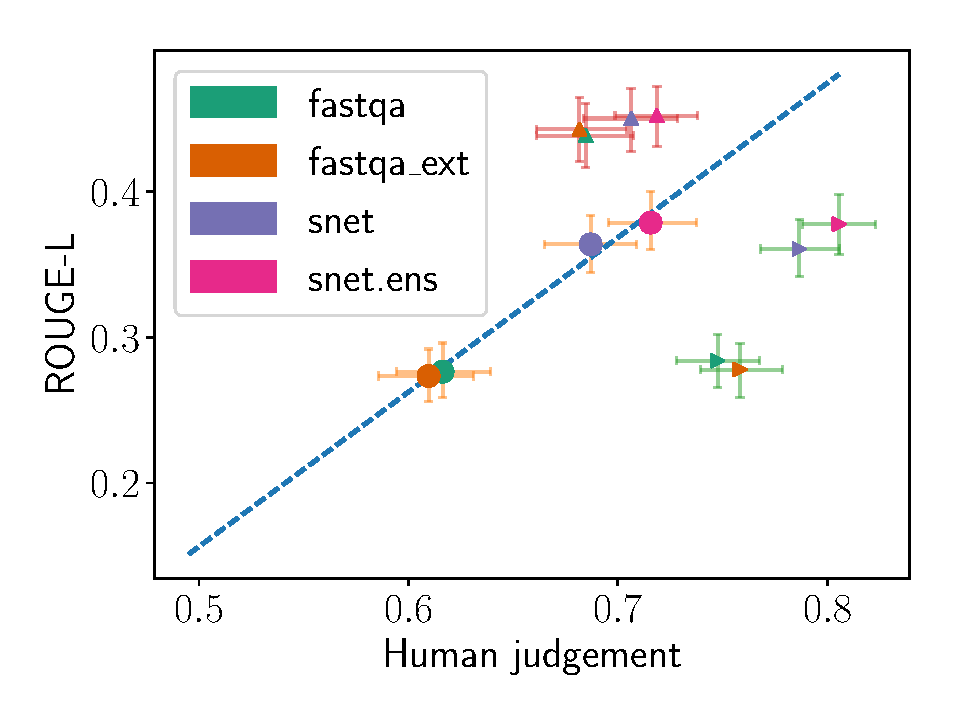
\includegraphics[width=0.8\textwidth]{figures/msmarco_bias}
    \caption{\label{fig:bias-msmarco-system} System-level correlation on the MS MARCO task}
  \end{subfigure}

  \begin{subfigure}{\textwidth}
    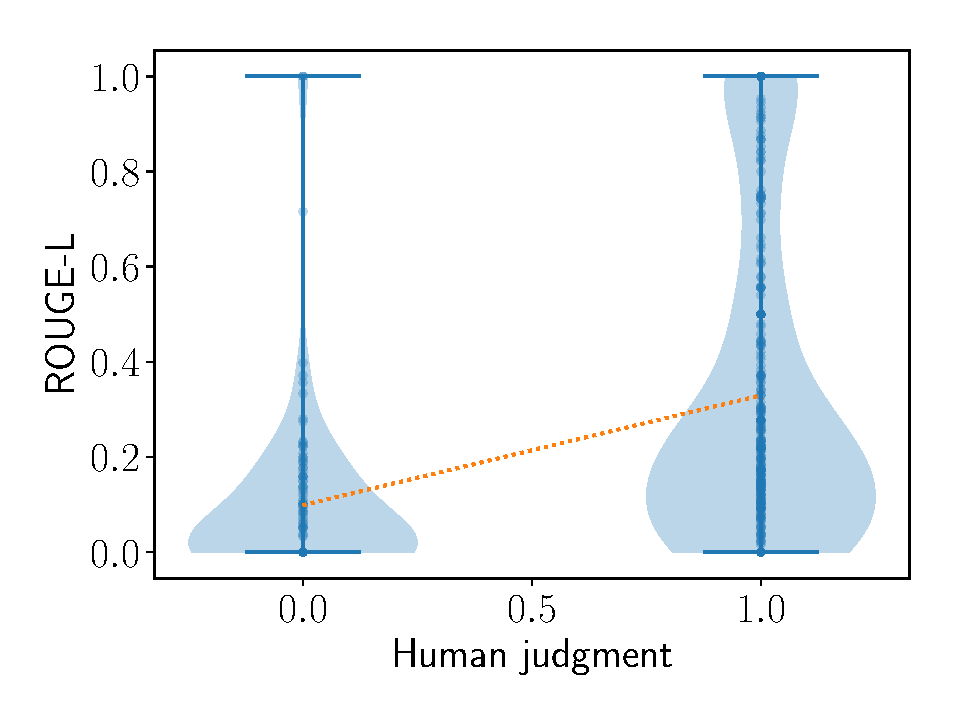
\includegraphics[width=0.8\textwidth]{figures/msmarco_instance_correlation}
    \caption{\label{fig:bias-msmarco-instance} Instance-level correlation for the \texttt{fastqa} system}
  \end{subfigure}

  \caption[System-level vs instance-level correlation on MS MARCO]{\label{fig:bias-msmarco}
  %We compare system-level and instance-level correlations between the ROUGE-L automatic metric and some human metric.
  (a) At a system-level, automatic metrics (ROUGE-L) and human judgment correlate well, but (b) the instance-level correlation plot
  (where each point is a system prediction) shows that the instance-level correlation is quite low ($\rho = 0.31$).
  %The instance-level correlation plot (where each point is an example) reveals that there is a large proportion of good answers that scored poorly by ROUGE, effectively ``hiding'' them from evaluation.
  As a consequence, if we try to locally improve systems to produce better answers ($\triangleright$ in (a)),
  they do not significantly improve ROUGE scores and vice versa ($\vartriangle$).
  %\pl{can we get rid of the left arrows to simplify / save space?}
  %At the same time, system changes that hurt human evaluation scores are not reflected by the automatic metric either (left arrows).
  %\ac{I don't know how to properly reference the fact that circles are systems and.} 
  }
\end{figure}


\section{\label{sec:bias} Bias in automatic evaluation}

% What does bias mean in natural language evaluation.
%The central theme of this paper is to bring to the fore a discussion of how we evaluate our generation systems.
%It is well understood that current automatic metrics are poorly correlated with human judgment at the instance-level~\citep{},
%yet, somewhat surprisingly they can still have high \textit{system-level} correlations~\citep{novikova2017why}.
%Does this imply that we should be able to assess system improvements?
%We will argue that high system-level correlations are insufficient.
%\ac{should I cite original ROUGE papers as basically indicating high system level correlations}
% PL: sure, but maybe not essential
% TODO: Change to a "as a result" using novikova results!

%use the automatic metric to compare systems and thus make incremental progress towards a better system.
%Is this the complete story?

%\begin{table*}
%  \input{examples.table}
%  \caption{\label{tab:examples} Examples on MS MARCO where the proposed answer is correct, but ROUGE-L is low
%  due to multiple correct answers.}
%\end{table*}

\begin{table}[!p]
  \centering
  \input{examples-1.table}
  \caption[Examples highlighting where automatic metric and human judgments agree or disagree on MS MARCO.]{\label{tab:examples-msmarco}
    Examples highlighting the different modes in which the automatic metric and human judgments may agree or disagree on the MS MARCO task.
    Human annotators rated answer correctness (\texttt{AnyCorrect}) and the automatic metric used is ROUGE-L (higher is better).
    A majority of responses from systems were actually correct but poorly scored according to ROUGE-L.
  }
\end{table}

\begin{table}[!p]
  \centering
  \input{examples-2.table}
  \caption[Examples highlighting where automatic metric and human judgments agree or disagree on CNN/Daily Mail.]{\label{tab:examples-cdm}
    Examples highlighting the different modes in which the automatic metric and human judgments may agree or disagree on the CNN/Daily Mail task.
    Human judgment scores used are post-edit distance (\texttt{Edit}) (lower is better) and the automatic metric used is sentence vector similarity with the reference (higher is better).
    A significant number of examples which are scored highly by VecSim are poorly rated by humans, and likewise many examples scored poorly by VecSim are highly rated by humans.
  }
\end{table}

It is well understood that current automatic metrics tend to correlate poorly with human judgment at the instance-level.
% Example 1: novikova 
For example, \citet{novikova2017why} report correlations less than $0.3$ for a large suite of word-based and grammar-based evaluation methods on a generation task.
% Example 2: Liu
Similarly, \citet{liu2016evaluate} find correlations less than $0.35$ for automatic metrics on a dialog generation task in one domain, but find correlations with the same metric dropped significantly to less than $0.16$ when used in another domain. 
Still, somewhat surprisingly, several automatic metrics have been found to have high \textit{system-level} correlations~\citep{novikova2017why}.
What, then, are the implications of having a low instance-level correlation?  

As a case study, consider the task of open-response question answering:
  here, a system receives a human-generated question and must \textit{generate} an answer from some given context, e.g.\ a document or several webpages.
  We collected the responses of several systems on the MS MARCOv1 dataset~\citep{nguyen2016ms} and crowdsourced human evaluations of the system output
  (see \refsec{tasks} for details).
%ROUGE-L and human judgment appear to be well correlated at the system-level (\reffig{bias-msmarco-system}) \stm{isn't this a bs claim since we really only have two systems? depend on references?},
%is high\footnote{%
  %The correlation measured between systems in \reffig{bias-system-msmarco} is $\rho = 0.99$, the correlation is computed with two pairs of similar systems and hence this correlation is not a fair estimate.} 

The instance-level correlation (\reffig{bias-msmarco-instance}) is only $\rho = 0.31$.
A closer look at the instance-level correlation reveals that
while ROUGE is able to correctly assign low scores to bad examples (lower left),
it is bad at judging good examples and often assigns them low ROUGE scores (lower right)---see \reftab{examples-msmarco} and \reftab{examples-cdm} for examples.
This observation agrees with a finding reported in \citet{novikova2017why} that automatic metrics correlate better with human judgments on bad examples than average or good examples. 

% PL: breaks the flow, so cut
%This observation was also made by \citet{novikova2017why} in the context of evaluating dialogue generation.
%Though variants of automatic metrics such as METEOR~\citep{lavie2009meteor} were designed
%to better capture linguistic variation they still have low correlation.

% Improve ROUGE, no human quality; improve human quality
Thus, as \reffig{bias-msmarco}(a) shows, we can improve low-scoring ROUGE examples without improving their human judgment ($\vartriangle$) and vice versa ($\triangleright$).
Indeed, \citet{conroy2008mind} report that summarization systems were optimized for ROUGE during the DUC challenge~\citep{dang2006overview}
until they were indistinguishable from the ROUGE scores of human-generated summaries, but the systems had hardly improved on human evaluation.
% PL: save space % we're under now and I think this is an important point
Hill-climbing on ROUGE can also lead to a system that does worse on human scores, e.g.\ in machine translation~\citep{wu2016google}.
Conversely, genuine quality improvements might not be reflected in improvements in ROUGE\@.
This bias also appears in pool-based evaluation for knowledge base population \citep{chaganty2017unbiased}.
Thus the problems with automatic metrics clearly motivate the need for human evaluation,
but can we still use the automatic metrics somehow to save costs?

% PL: I like this, but I think we don't have space to explain it properly
%These are interesting examples that we would like our systems to be able to handle,
%but because automatic metrics correlate so poorly on this subset, they are in effect ``hidden'' from our evaluation.
%To demonstrate this point, we took each system in our earlier experiment and swapped any output that is scored poorly by ROUGE with that of another system
%to do either better (left arrow) or worse (right arrow) than the original output as evaluated by humans.
%The ROUGE scores of the perturbed systems remain the same while the human evaluation scores are significantly affected.
%On the other hand, if we perturbed the input to only improve the ROUGE scores of examples which scored poorly on ROUGE scores (up arrow),
%we see essentially no improvements in human judgment scores.
%they found that as systems tuned using ROUGE they successively improved on the automatic metric until they were indistinguishable from human performance while still hardly budging on human evaluations.

% Conclusion:
%   - simply having high system-level correlations is insufficient for a metric.
%   - instead, we should strive to meet human judgment and be unbiased statistically.
%The ramifications of this are that if we were to make a genuine improvement in a system
%that happens to improve upon difficult examples (i.e.\ move more output to the lower right corner),
%we would not observe any improvement in ROUGE and are likely not to pursue such a direction further.\@
%Indeed, \citet{conroy2008mind} report that as summarization systems tuned using the ROUGE metric for the DUC challenge~\citet{},
%they successively improved on the automatic metric until they were indistinguishable from human ROUGE scores while hardly budging on human evaluations.

%\stm{The points made in the next couple sentences are pretty weak and vague. You mention much more convincing points in the Related Work. Can you put some of those here?}
%This gap between improving automatic metric scores and human evaluation scores was also observed by  when comparing the performance of summarization systems in the DUC summarization challenges~\citep{} across years.
%In fact there is already bias: systems that exist in the literature
%are likely to have high human-automatic correlation since that's how they have been developed.
%\pl{not sure if this solid}
% PL: wanted to talk about genuine improvements

%\ac{I don't know how to end this section yet. I want it to lead into our approach of being unbiased.}

%Thus, we should care not about finding automatic metrics that have high
%system-level correlations with human judgments, but rather ways of actually
%measuring human judgment better.
%\pl{a bit too preachy}
%This is what we mean by unbiased!

% - Statistically, it's not equal to what we posit.
% - Practically, it means that the evaluation systematically favors one set of systems over another.
% - Understandable when system-level correlation is low, but should high system-level correlations simply be the goal of evaluation metrics?
% - We argue not.
